%%%%%%%%%%%%%%%%%%%%%%%%%%%%%%%%%%%%%%%%%%%%%%%%%%%%%%%%%%%%%%%%%%%%%%
% CS2030S Midterms Cheatsheet
% Author: San Diego John Michael Bautista
%%%%%%%%%%%%%%%%%%%%%%%%%%%%%%%%%%%%%%%%%%%%%%%%%%%%%%%%%%%%%%%%%%%%%%

\documentclass[10pt,landscape]{article}
\usepackage{amssymb,amsmath,amsthm,amsfonts}
\usepackage{multicol,multirow}
\usepackage{calc}
\usepackage{ifthen}
\usepackage{fancyvrb}
\usepackage{listings}
\usepackage{longtable}
\usepackage[landscape]{geometry}
\usepackage[colorlinks=true,citecolor=blue,linkcolor=blue]{hyperref}
\usepackage{mdframed}
\usepackage{graphicx}
\graphicspath{{./images/}}

\ifthenelse{\lengthtest { \paperwidth = 11in}}
{ \geometry{top=.5in,left=.5in,right=.5in,bottom=.5in} }
{\ifthenelse{ \lengthtest{ \paperwidth = 297mm}}
    {\geometry{top=1cm,left=1cm,right=1cm,bottom=1cm} }
    {\geometry{top=1cm,left=1cm,right=1cm,bottom=1cm} }
}
\pagestyle{empty}
\makeatletter
\renewcommand{\section}{\@startsection{section}{1}{0mm}%
    {-1ex plus -.5ex minus -.2ex}%
    {0.5ex plus .2ex}%x
    {\normalfont\large\bfseries}}
\renewcommand{\subsection}{\@startsection{subsection}{2}{0mm}%
    {-1explus -.5ex minus -.2ex}%
    {0.5ex plus .2ex}%
    {\normalfont\normalsize\bfseries}}
\renewcommand{\subsubsection}{\@startsection{subsubsection}{3}{0mm}%
    {-1ex plus -.5ex minus -.2ex}%
    {1ex plus .2ex}%
    {\normalfont\small\bfseries}}
\makeatother
\setcounter{secnumdepth}{0}
\setlength{\parindent}{0pt}
\setlength{\parskip}{0pt plus 0.5ex}

% -----------------------------------------------------------------------

\title{CS2030S Midterms CheatSheet}

\begin{document}

\raggedright
\footnotesize

\begin{center}
    \Large{\textbf{CS2030S Midterms Cheatsheet}} \\
    by @jmsandiegoo
\end{center}
\begin{multicols*}{3}
    % \setlength{\premulticols}{1pt}
    % \setlength{\postmulticols}{1pt}
    % \setlength{\multicolsep}{1pt}
    \setlength{\columnsep}{2pt}

    \begin{mdframed}
        \section{2. Variable Type}
    \end{mdframed}
    \subsection{Data Abastraction: Variables}
    A variable is an abstraction that allows us to give a user-friendly name to a piece of data in memory

    \subsection{Static Type}
    Variables type are declared during compile time. A variable can only hold values of same type and cannot be changed.
    \subsection{Primitive Types \& Subtyping}
    \begin{Verbatim}[xleftmargin=-.45in]
        byte (0) <: short (0) <: int (0) <: long (0L)
        <: float (0.0f) <: double (0.0d)

        char ('\u0000') <: int

        boolean (false)
    \end{Verbatim}
    \textit{* Primitive type never share their value with each other}
    \subsection{Reference Types}
    \begin{Verbatim}[xleftmargin=-.45in]
        classes (null)
    \end{Verbatim}
    \textit{* Reference type share their value with each other}

    \begin{mdframed}
        \section{3. Functions}
    \end{mdframed}
    \subsection {Abstraction (Computation) Function}
    Function allows:
    \begin{itemize}
        \item Compartmentalize computation
              \begin{itemize}
                  \item complexity and variables only within the function body and doesn't affect outside code
              \end{itemize}
        \item Hide implementation
              \begin{itemize}
                  \item caller only need to worry what the function does (parameters and return)
                  \item does not affect caller when code evolves and changes overtime
              \end{itemize}
        \item Reduce repetition
              \begin{itemize}
                  \item can just call the function with varying parameters to conduct same computation for diff values
                  \item also any changes can be done in one place which is the function itself
              \end{itemize}
    \end{itemize}
    \subsection{Abstraction Barrier}
    A barrier between the code that calls \textbf{(by: client)} the function and the code that implements/define the function \textbf{(by: implementer)}.
    \medskip
    \begin{mdframed}
        \section{4. Encapsulation}
    \end{mdframed}
    \subsection{Abstraction: Composite Data Types}
    Group primitive types together and abstracts it away allowing us to think at higher level of conceptualization
    \begin{lstlisting}[language=Java, xleftmargin=-.3in]
    typedef struct {
        double x, y; // coordinate of center.
        double r; // radius
        } circle;
    \end{lstlisting}

    \textit{* Usually has corresponding functions that uses the struct to completely be shielded from the representation}

    \subsection{Abstraction: Class a.k.a Encapsulation}
    Abstracts composite type and associated functions on the same side of abstraction barrier
    \\ Consists of data fields/members/states/attributes \& methods
    \begin{lstlisting}[language=Java, xleftmargin=-.3in]
    class Circle {
        double x;
        double y;
        double r;
        
        double getArea() {
            return 3.141592653589793 * r * r;
        }
    }
    \end{lstlisting}

    \begin{mdframed}
        \section{5. Information Hiding}
    \end{mdframed}
    Use of access modifiers to prevent field or method access from outside class / abstraction barrier

    \subsection{Constructors}
    \begin{lstlisting}[language=Java, xleftmargin=-.3in]
    // inside Circle class
    public Circle(double x, double y, double r) {
        this.x = x;
        this.y = y;
        this.r = r;
    } 
    // outside
    Circle c = new Circle(0.0, 0.5, 10.0);
    \end{lstlisting}

    \begin{mdframed}
        \section{6. Tell Don't Ask}
    \end{mdframed}
    \subsection{Accessor / Getter \& Mutator / Setter}
    A public method in class that retrieves and updates the value of the field.
    \\ \textit{* Harmful, exposes internal representation. Still can be used in "no choice" scenarios}
    \subsection{Tell Don't Ask Principle}
    Client tells the circle what to do, instead of asking for its fields
    \begin{lstlisting}[language=Java, xleftmargin=-.3in]
    // wrong
    double cX = c.getX();
    double cY = c.getY();
    double r = c.getR();
    boolean isInCircle = 
        ((x - cX) * (x - cX) + 
        (y - cY) * (y - cY)) <= r * r;
    // correct
    boolean isInCircle = c.contains(x, y);
    \end{lstlisting}

    \begin{mdframed}
        \section{7-8. Class Fields \& Methods}
    \end{mdframed}
    \subsection{Class Fields}
    Useful for sharing shared values across class instances
    \begin{lstlisting}[language=Java, xleftmargin=-.3in]
    class Math {
        :
        public static final double PI = 3.141...;
        :
    }
    // access
    Math.PI;
    \end{lstlisting}
    \textit{* \textbf{final} means cannot be changed / constant}
    \subsection{Class Methods}
    A method that is independent of an instance. Has no \textbf{this} reference
    \begin{lstlisting}[language=Java, xleftmargin=-.3in]
    class Circle {
        :
        // can only access static fields
        public static int getNumOfCircles() {
            return Circle.lastId; 
        }
        :
    }
    
    // main program entry point
    public final static void main(String[] args) {
        :
    }
    \end{lstlisting}

    \newpage
    \begin{mdframed}
        \section{9. Composition}
    \end{mdframed}
    Models a HAS-A relationship, enables further layer of abstraction and maintability.
    \begin{lstlisting}[language=Java, xleftmargin=-.3in]
    class Circle {
        private Point c;   // HAS-A Point (center)
        private double r;  // the length of radius
        :
    }
    \end{lstlisting}
    HAS-A can have shared
    \begin{mdframed}
        \section{10. Heap \& Stack}
    \end{mdframed}
    \subsection{Type of Calls}
    Primitive Types: call by value
    \\Reference Types: call by reference

    JVM Memory parititions:
    \begin{itemize}
        \item \textbf{method area}: stores method codes
        \item \textbf{metaspace}: stores meta information of class
        \item \textbf{heap}: stores dynamically allocated objects
        \item \textbf{stack}: stores local variables
    \end{itemize}

    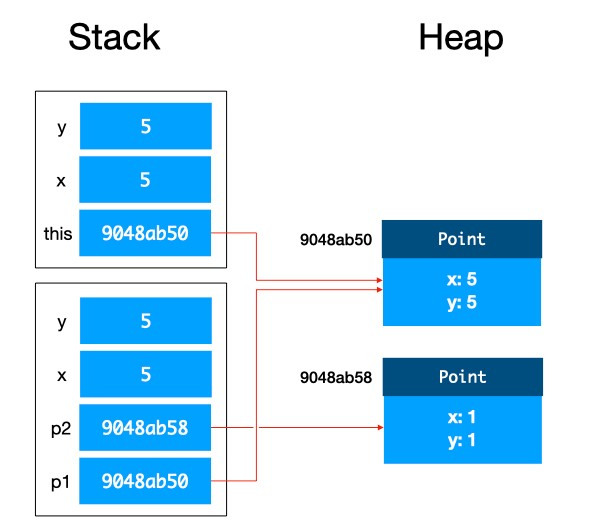
\includegraphics[width=\linewidth]{heap_stack}
    \textit{* Don't forget label the stack frames \& the main method args variable and array}
    \begin{mdframed}
        \section{11 - 13. Inheritance, Overriding \& Overloading}
    \end{mdframed}
    \subsection{Inheritance}
    Models a IS-A relationship, enables classes to have a parent-child relationship.
    \begin{itemize}
        \item \textbf{Child (subclass)}: has all the parent's and its own unique characteristics (extends)
        \item \textbf{Parent (parebt/super class)}: the more general object where the child is basing from
    \end{itemize}
    \begin{lstlisting}[language=Java, xleftmargin=-.3in]
    // version 0.3 (using inheritance)
    class ColoredCircle extends Circle {
        private Color color;
    
        public ColoredCircle(Point center, 
            double radius, 
            Color color) {
        // call the parent's constructor
        super(center, radius);  
        this.color = color;
        }
    }
    \end{lstlisting}
    \subsection{Run-Time vs Compile-Time Type}
    \begin{lstlisting}[language=Java, xleftmargin=-.3in]
    Circle c = new ColoredCircle(p, 0, blue);
    \end{lstlisting}
    Compile-time Type is the type of the var c during compilation which is Circle
    \smallskip
    \\Run-Time Type is the type of the var c during runtime which is ColoredCircle
    \\ \textit{* All classes inherits from Object}
    \subsection{Overriding}
    Overriding allows child class to change the inherited method behaviour. Subclass can override with same method descriptor
    \\ \textbf{Method Signature}: method name and the number, type, and order of its parameters
    \\ \textbf{Method Descriptor}: method signature + return type
    \begin{lstlisting}[showstringspaces=false, language=Java, xleftmargin=-.3in]
    class Circle {
        :
       // hints compiler overriding occurs
       // so compiler will help us check
       // also return type can subtype
       @Override
       public String toString() {
           return "{ center: " + 
            this.c + ", radius: " + this.r + " }";
       }
    }
    \end{lstlisting}
    \textit{* super can be used to call overridden methods}
    \subsection{Overloading}
    Allows to define multiple methods of same name but different method signature. Also
    \\ \textit{* Cannot overload with different return type}

    \begin{mdframed}
        \section{14. Polymorphism}
    \end{mdframed}
    Method overriding and dynaminc typing allows polymorphism to occur.
    An obj can have many forms (takes form of its many subtypes) in which
    its method is invoked depending run-time type (dynamic binding only works for non static methods).
    \begin{lstlisting}[showstringspaces=false, language=Java, xleftmargin=-.3in]
    // version 0.1 (with polymorphism)
    boolean contains(Object[] array, Object obj) {
        for (Object curr : array) {
            // Polymorphism
            if (curr.equals(obj)) {
            return true;
            }
        }
        return false;
    }
    \end{lstlisting}

    \begin{mdframed}
        \section{15 - 16. Method Invocation \& LSP}
    \end{mdframed}
    \subsection{Method Invocation}
    Identifies which method implementation to be executed. Two step process:
    \begin{enumerate}
        \item \textbf{Compile Time}: Identify the target's compile-time type, find and store
              closest method descriptor for the method invoked.
              \\ \textit{* choose the most specific method that accepts N $<$: M}

        \item \textbf{Run Time}: Identify target's run-time type and search from run-time type up
              the hierarchy. Execute the first matched method.
    \end{enumerate}
    \textit{* class methods don't apply here}

    \subsection{Liskov Substitution Principle}
    $S <: T$, states that code using type $T$ if substituted with $S$ should still work and pass the test cases.
    $S$ should not change the overal behaviour of $T$
    \\\textit{* use final for class and method to prevent inheritance and overriding }
    \newpage
    \begin{mdframed}
        \section{17 - 18. Abstract Class \& Interface}
    \end{mdframed}
    \subsection{Abstract class}
    A class that is too general to have all method defined
    \\It cannot be instantiated
    \\Not all methods have to be abstract
    \begin{lstlisting}[showstringspaces=false, language=Java, xleftmargin=-.3in]
    abstract class Shape {
        :
        // subclasses must implement this
        abstract public double getArea();
    }
    \end{lstlisting}

    \subsection{Interface}
    Models "can do" behaviour. To group classes not necessarily "IS-A" but with same "do"
    behaviour.
    \begin{itemize}
        \item Class can only extend from one class but can implement multiple interfaces
        \item Interface can extend from multiple interfaces but not from class
    \end{itemize}
    \begin{lstlisting}[showstringspaces=false, language=Java, xleftmargin=-.3in]
    interface GetAreable {
        public abstract double getArea();
    }

    abstract class Shape implements GetAreable {
        :
    }

    class Flat extends RealEstate 
        implements GetAreable {
        :
        @Override
        public double getArea() {
            :
        }
    }  
    \end{lstlisting}
    \subsection{Interface Casting}
    \begin{lstlisting}[showstringspaces=false, language=Java, xleftmargin=-.3in]
    interface I {
    :
    }
    class A {}
    class B implements I {}
    // Compiles, widening type conversion
    I i1 = new B();
    // Also compiles, as subtype could implement
    // interface
    I i2 = (I) new A();
    \end{lstlisting}
    \begin{mdframed}
        \section{19. Wrapper Class}
    \end{mdframed}
    Wraps primitive types to its corresponding class.
    \begin{lstlisting}[showstringspaces=false, language=Java, xleftmargin=-.3in]
    Integer i = new Integer(4) 
    int j = i.intValue();
    // with auto-boxing/unboxing
    Integer i = 4;
    int j = i;
    // can also unbox and widen to other primitive
    \end{lstlisting}
    \textit{* less performant terms of heap space and immutability as a result of auto-box}

    \begin{mdframed}
        \section{20 - 21. Casting \& Variance}
    \end{mdframed}
    \subsection{Casting}
    \begin{itemize}
        \item \textbf{Widening type conversion}: done implicitly

        \item \textbf{Narrowing type conversion}: explicit and must be careful of as it could
              cause run-time errors
              \begin{lstlisting}[showstringspaces=false, language=Java, xleftmargin=-1.2in]
                // Circle <: GetAreable
                // ok
                GetAreable ga = findLargest(circles);
                // ok
                Circle c2 = (Circle) findLargest(circles);
              \end{lstlisting}
    \end{itemize}
    \subsection{Variance}
    Refers to the subtyping relationship between complex types like arrays
    \begin{itemize}
        \item \textbf{covariant}: $S <: T$ implies $C(S) <: C(T)$
        \item \textbf{contravariant}: $S <: T$ implies $C(T) <: C(S)$
        \item \textbf{invariant}: neither of the two
    \end{itemize}
    \textit{* Java array is covariant}
    \begin{mdframed}
        \section{22. Exception}
    \end{mdframed}
    \subsection{Catching exception}

    \begin{lstlisting}[showstringspaces=false, language=Java, xleftmargin=-.3in]
    try {
        // do something
        reader = new FileReader(filename);
        scanner = new Scanner(reader);
        value = scanner.nextInt();
    }
    // (Exception1 | Exception2 e)
    catch (FileNotFoundException e) {
        // handle exception
        System.err.println("Unable to open");
    }
    finally {
        // clean up code
        // would still run even after 
        // return or throw
        if (scanner != null)
            scanner.close();
    }
    \end{lstlisting}

    \subsection{Throwing / Passing Exception}
    \begin{lstlisting}[showstringspaces=false, language=Java, xleftmargin=-.3in]
    // throws after params
    public Circle(Point c, double r) 
        throws IllegalArgumentException {
        if (r < 0) {
            throw new IllegalArgumentException(
            "radius cannot be negative.");
        }
        this.c = c;
        this.r = r;
    }
    // can also catch it inside function
    // if just pass the buck no throw would occur
    // just throws keyword after function params
    \end{lstlisting}
    \subsection{Checked vs Unchecked}
    \textbf{Checked $<:$ Exception}: an exception that a programmer has no control over with despite
    no error in code. MUST BE CHECKED AND HANDLED if not won't compile.
    \\\textbf{Unchecked $<:$ RuntimeException}: exception caused my programmer's mistake in the code. NOT EXPLICITLY
    CAUGHT / THROWN. Leads to runtime errors
    \subsection{Control Flow}
    When an exception is thrown instruction after it will not be executed. Instead the caller that catch and handles the error
    will be passed the control flow of the program.
    \subsection{Creating Own Exception}
    Own excpetion can be created by extending the existing Java Exception classes.
    \subsection{Override Method Throwing Exception}
    Can be overriden but make sure the method throws the same or a subclass of the exception thrown
    \subsection{Best Practices}
    \begin{itemize}
        \item Catch Exceptions to Clean Up
        \item Do not catch-them-all!
        \item Overreacting: don't terminate when exception is catched
        \item Do Not Break Abstraction Barrier
        \item Do NOT Use Exception As a Control Flow Mechanism
    \end{itemize}

    \newpage
    \begin{mdframed}
        \section{23 - 24. Generics \& Type Erasure}
    \end{mdframed}
    \subsection{Generic Class}
    \begin{lstlisting}[showstringspaces=false, language=Java, xleftmargin=-.3in]
    // <> type parameter
    // compiler can also type check
    class Pair<S,T> {
        private S first;
        private T second;
        
        public Pair(S first, T second) {
            this.first = first;
            this.second = second;
        }
        
        S getFirst() {
            return this.first;
        }
        T getSecond() {
            return this.second;
        }
    }
    // passing T parameter to another generic
    class DictEntry<T> extends 
        Pair<String,T> {
        :
    }
    // once type args passed it is now 
    // parameterized type
    Pair<String,Integer> p = 
        new Pair<String,Integer>("hello", 4);
    \end{lstlisting}
    \subsection{Bounded Parameters \& Generic Methods}
    \begin{lstlisting}[showstringspaces=false, language=Java, xleftmargin=-.3in]
    class A {
        // version 0.5
        // extends even supertype is interface
        // extends also works if T is GetAreable
        public static <T extends GetAreable> 
            T findLargest(T[] array) {
            double maxArea = 0;
            T maxObj = null;
            for (T curr : array) {
                double area = curr.getArea();
                if (area > maxArea) {
                    maxArea = area;
                    maxObj = curr;
                }
            }
            return maxObj;
        }
    }
    \end{lstlisting}
    \textit{* bounded params can be used for declaring generic classes as well}
    \subsection{Type Erasures}
    Java takes a code sharing approach, it erase the type parameters and type arguments during compilation (after type checking).
    \begin{lstlisting}[showstringspaces=false, language=Java, xleftmargin=-.3in]
    class Pair {
        private Object first;
        private Object second;
        
        public Pair(Object first, Object second) {
            this.first = first;
            this.second = second;
        }
        
        Object getFirst() {
            return this.first;
        }
        
        Object getSecond() {
            return this.second;
        }
    }
    \end{lstlisting}
    \subsection{Arrays and Generics don't mix}
    Leads to heap pollution as generics is not refiable
    \begin{lstlisting}[showstringspaces=false, language=Java, xleftmargin=-.3in]
    // create a new array of pairs
    Pair<String,Integer>[] pairArray = 
        new Pair<String,Integer>[2];
    
    // pass around the array of pairs 
    // as an array of object
    Object[] objArray = pairArray;
    
    // put a pair into the array 
    // -- no ArrayStoreException!
    objArray[0] = 
        new Pair<Double,Boolean>(3.14, true);
    
    // Realistiacally these are illegal
    new Pair<S,T>[2];
    new T[2];
    \end{lstlisting}
    \begin{mdframed}
        \section{25. Unchecked Warnings}
    \end{mdframed}
    Unchecked warning means that compiler could not help us detect possible run-time
    exceptions (ClassCastException) due to type erasures.
    \begin{lstlisting}[showstringspaces=false, language=Java, xleftmargin=-.3in]
    class Array<T> {
        private T[] array;

        Array(int size) {
            // leave a reason note
            // min scope and only declarations
            // ensure no error would occur
            @SuppressWarnings("unchecked")
            // throws unchecked as it may have
            // items that are not type T
            T[] a = (T[]) new Object[size];
            this.array = a;
        }

        public void set(int index, T item) {
            this.array[index] = item;
        }

        public T get(int index) {
            return this.array[index];
        }
    }
    \end{lstlisting}

    \subsection{Raw Types}
    Using generic types without type arguments will also lead to run-tme errors.
    \begin{mdframed}
        \section{26. Wildcards}
    \end{mdframed}
    \subsection{Upper-Bounded Wildcards}
    \begin{lstlisting}[showstringspaces=false, language=Java, xleftmargin=-.3in]
    // ? can be substituted with S 
    // or subtype of it

    Array<? extends S>

    // upper-bound is covariant
    Array<C> <: Array<? extends C>

    C <: S, Array<? extends C> <: Array<? extends S>

    Array<C> <: Array<? extends S> (transitive)

    \end{lstlisting}
    \subsection{Lower-Bounded Wildcards}
    \begin{lstlisting}[showstringspaces=false, language=Java, xleftmargin=-.3in]
    // ? can be substituted with S 
    // or supertype of it

    Array<? super S>

    // lower-bound contravariant
    Array<S> <: Array<? super S>
    C <: S, Array<? super S> <: Array<? super C>
    Array<S> <: Array<? super C> (transitive)
    \end{lstlisting}
    \subsection{Producer Extends Consumer Super (PECS)}
    Producer: returns variable of type T $<?\, extends\, T>$
    Consumer: takes in a variable of type T $<?\, super\, T>$
    \subsection{Unbounded Wildcards}
    Supertype of all parameterezied type
    \begin{lstlisting}[showstringspaces=false, language=Java, xleftmargin=-.3in]
    // ? can be substituted with any type
    // array of objects of some specific, 
    // but unknown type
    Array<?>

    // array of object, with
    // typchecking by the compiler
    Array<Object>

    // array of Object instances, 
    // without type checking.
    Array

    // Can be used with instanceof
    a instanceof A<?> 
    // Can be used with array
    T[] a = (T[]) new Comparable<?>[size]

    \end{lstlisting}
    \begin{mdframed}
        \section{27. Type Inference}
    \end{mdframed}
    \subsection{Diamond Operator}
    Java helps infer the parameter types of the generic when instantiating a new instance.
    \begin{lstlisting}[showstringspaces=false, language=Java, xleftmargin=-.3in]
    // inferred the new instance as
    // type Pair<String, Integer>
    Pair<String,Integer> p = new Pair<>();
    \end{lstlisting}
    \subsection{Target Typing}
    \begin{enumerate}
        \item Identify Target Typing
        \item Identify Argument Typing
        \item Bounds on Typing
    \end{enumerate}
    \textit{* Lowest Bound is taken}
\end{multicols*}
\end{document}
